% ===== File: final_report.tex =====
% EECS 570 Term Project Final Report (Winter 2026)
\PassOptionsToPackage{table}{xcolor}
\documentclass[10pt,twocolumn]{article}

\usepackage[margin=0.75in]{geometry}
\usepackage{booktabs}
\usepackage{enumitem}
\usepackage{amsmath}
\usepackage{amssymb}
\usepackage{graphicx}
\graphicspath{{../}{./}}
\usepackage{colortbl}
\usepackage{xcolor}
\usepackage{caption}
\usepackage{subcaption}
\usepackage{tikz}
\usepackage[hidelinks]{hyperref}
\usepackage{titling}
\usetikzlibrary{arrows.meta,positioning,shapes.geometric,calc}
\setlist{nosep,leftmargin=*}

\renewcommand{\abstractname}{\vspace{-\baselineskip}}

% ── Color definitions ─────────────────────────────────────────────────────────
\definecolor{umblue}{RGB}{0,39,76}
\definecolor{ummaize}{RGB}{255,203,5}
\definecolor{supported}{RGB}{34,139,34}
\definecolor{partial}{RGB}{180,120,0}
\definecolor{refuted}{RGB}{178,34,34}

\newcommand{\cpasync}{\texttt{cp.async}}
\newcommand{\highlight}[1]{\colorbox{ummaize!35}{\textbf{#1}}}
\newcommand{\wconc}{W_{\text{conc}}}
\newcommand{\cleff}{C_{\text{L2}}^{\text{eff}}}
\newcommand{\Leff}{L_{\text{eff}}}
\newcommand{\LLtwo}{L_{\text{L2}}}
\newcommand{\Ldram}{L_{\text{DRAM}}}
\newcommand{\Tcomp}{T_{\text{comp}}}
\newcommand{\Smin}{S_{\min}}

% ── Title & authors ───────────────────────────────────────────────────────────
\begin{document}

\title{\vspace{-2ex}\Large\bfseries Predicting \cpasync{} Pipeline Effectiveness from\\
Memory-Subsystem Parameters: A Cross-GPU Study\\[2pt]
\normalsize\mdseries\itshape EECS 570 Term Project Final Report, Winter 2026}

\author{}
\date{}

\twocolumn[\begin{@twocolumnfalse}
\maketitle
\vspace{-5ex}
\begin{center}
\begin{tabular}{cc}
Xiangchen Song & Chenxin Geng \tabularnewline
University of Michigan -- Ann Arbor & University of Michigan -- Ann Arbor \tabularnewline
\texttt{xxxchen@umich.edu} & \texttt{gchenxin@umich.edu} \tabularnewline
\noalign{\vskip 8pt}
Yuyang Feng & Tian Xia \tabularnewline
University of Michigan -- Ann Arbor & University of Michigan -- Ann Arbor \tabularnewline
\texttt{yuyangfe@umich.edu} & \texttt{crazyjoe@umich.edu}
\end{tabular}
\end{center}
\vspace{1em}
\begin{quote}\small
\noindent\textbf{Abstract.}\quad
NVIDIA's \cpasync{} instruction (Ampere SM80 and later) enables
asynchronous global-to-shared pipelined copies that are central to
CUTLASS, FlashAttention-3, and Triton.  Practitioners routinely tune
pipeline depth $S$ on one GPU and reuse it elsewhere.  We test this
assumption by running identical \cpasync{} kernels (FP32 GEMM and a
1-D stencil) on five GPUs across four architectures (V100, A40,
A100~MIG~3g.40gb, L40S, H100~SXM5).  \emph{(i)}~Best-case GEMM
speedup vs.\ a naive global-memory baseline ranges from
$\sim$1.0$\times$ (L40S) to $\sim$1.20$\times$ (H100) on the same
source, invalidating portability.  \emph{(ii)}~A pointer-chase sweep shows H100's 50\,MB L2 yields
only 26\,MB effective due to slice locality, while other tested
GPUs' plateaus match nominal capacity.
\emph{(iii)}~A predictive model combining an L2-aware latency
estimate, an empirically calibrated 280-cycle per-stage overhead
floor, and a sub-linear ($\alpha{=}0.15$) occupancy penalty attains
\highlight{9.0\% GEMM MAPE} and \highlight{5.2\% stencil MAPE}
across the four \cpasync{}-capable GPUs with no kernel-data fitting.
\emph{(iv)}~A Triton autotune pre-filter prunes 60--67\% of a
96-config GEMM grid; it is intended as a coarse pass before
exhaustive benchmarking.
\end{quote}
\vspace{1em}
\end{@twocolumnfalse}]

% ============================================================
\section{Introduction}
\label{sec:intro}
% ============================================================

Hiding global-memory latency is central to GPU kernel optimisation.
NVIDIA's \cpasync{} instruction (Ampere, SM80) copies data from
global to shared memory bypassing the register file, and is
software-pipelined using a commit/wait protocol~\cite{cuda_guide}.
CUTLASS~3.x~\cite{cutlass3}, FlashAttention-3~\cite{flashattn3}, and
Triton~\cite{triton} all rely on multi-stage \cpasync{} pipelines;
the \emph{pipeline depth} $S$ is one of the key tuning knobs.

\paragraph{Portability gap.}
Depth is tuned once per kernel and assumed to transfer across GPUs
sharing the instruction.  Yet pipeline effectiveness is not a pure
ISA property: it depends on L2 capacity, memory latency/bandwidth,
and per-SM shared memory---all of which vary by $>$10$\times$ even
among \cpasync{}-capable GPUs.  No prior study has quantified how
this variation affects optimal $S$, and no autotuner uses
architecture parameters to prune the grid before exhaustive search.

\paragraph{Research question.}
\emph{Does the optimal depth $S^*$ and its marginal speedup diverge
across GPUs with different memory subsystems?  Can a lightweight
model predict this divergence from architecture constants alone and
thereby reduce autotuning cost?}

\paragraph{Approach.}
We implement FP32 GEMM and a 1-D stencil in three variants: V0
(naive global-memory), V1 (synchronous tiled), and V3 ($S$-stage
\cpasync{} ring buffer with identical tile geometry to V1).  The V3
source compiles unchanged on every \cpasync{}-capable GPU.  We run
the same code on five GPUs (V100, A40, A100~MIG~3g.40gb, L40S,
H100~SXM5), characterise each L2 with pointer chasing, construct a
three-term model, and validate by MAPE, leave-one-out, and
component-wise ablation.

\paragraph{Contributions.}
\emph{(1)}~A controlled cross-GPU \cpasync{} comparison on identical
source over five GPUs and two workloads.
\emph{(2)}~A pointer-chase characterisation including a first
MIG-instance measurement and a quantification of H100's
slice-locality cliff (50\,MB$\to$26\,MB effective).
\emph{(3)}~A two-constant predictive model (280-cycle floor,
$\alpha{=}0.15$, calibrated once and reused across GPUs) achieving
$\sim$9\% MAPE with no per-GPU refit; removing the floor raises
stencil MAPE to 157\%.
\emph{(4)}~A Triton autotune pre-filter pruning 60--67\% of a
96-config GEMM grid as a coarse pre-pass before exhaustive
benchmarking.

% ============================================================
\section{Background and Related Work}
\label{sec:related}
% ============================================================

\paragraph{\cpasync{} and pipeline studies.}
Introduced in Ampere (SM80), \cpasync{} issues a non-blocking
global$\to$shared copy bypassing the register file~\cite{cuda_guide};
committed/waited via \texttt{commit\_group}/\texttt{wait\_group}.
The same instruction is supported on Ada (SM89) and Hopper (SM90),
where TMA supersedes it for some uses~\cite{hopper_ieee,hopper_microbench}.
Li et al.~\cite{dtcspmm} show $>$2$\times$ from double-buffered
\cpasync{} pipelines for SpMM on Ampere; Chen et al.~\cite{tawa}
sweep depth on H100 revealing occupancy--depth trade-offs; Wu et
al.~\cite{twill} note that optimal pipelining relies on ``brittle
heuristics.''  Our study sweeps five GPUs with the same source and
offers a specification-based alternative to these heuristics.

\paragraph{L2 characterisation and autotuning.}
The roofline model~\cite{roofline} relates arithmetic intensity to
attainable throughput via the ridge point $R = F_{\text{peak}} /
\text{BW}_{\text{peak}}$; we use per-GPU $R$ for cross-GPU
normalisation (Table~\ref{tab:gpus}).  Mei and
Chu~\cite{mei_dissecting} establish the pointer-chase methodology;
Jin et al.~\cite{gpu_noc} reverse-engineer GPU NoC topology,
finding $<$70\% L2-latency variation from SM-to-slice
distance---which we independently confirm on H100.  Wei et
al.~\cite{hytis} model L2-aware GEMM scheduling but not
async-pipeline interaction.  Guo et al.~\cite{tritonblas} and
ACTA~\cite{acta} propose analytical Triton/Hopper parameter
selectors for a single GPU; Triton's
\texttt{@triton.autotune}~\cite{triton} is exhaustive.  Ernst et
al.~\cite{layer_conditions} identify cache ``layer conditions'' at
capacity thresholds---our L2-hit term is a concrete instance.  No
prior work characterises L2 under MIG partitioning~\cite{mig_guide}.

% ============================================================
\section{Experimental Setup}
\label{sec:setup}
% ============================================================

\subsection{Hardware}

\begin{table*}[t]
\centering
\small
\caption{Target GPUs.  Ridge $R$ in FLOP/byte.  L2 eff./$\LLtwo$/$\Ldram$
are pointer-chase outputs (Section~\ref{sec:microbench}); nominal
from \texttt{cudaDeviceProp}.  Latencies in cycles.}
\label{tab:gpus}
\renewcommand{\arraystretch}{1.15}
\begin{tabular}{@{}lccccc@{}}
\toprule
 & \textbf{V100} & \textbf{A40} & \textbf{A100 MIG} & \textbf{L40S}
 & \textbf{H100} \\
\midrule
Arch / SM ver.   & Volta/70 & Ampere/86 & Ampere/80 & Ada/89 & Hopper/90 \\
\cpasync{} / SMs & ---/80 & \checkmark/84 & \checkmark/42 & \checkmark/142 & \checkmark/132 \\
Mem.\ tech./size & HBM2/32\,GB & GDDR6/48\,GB & HBM2e/40\,GB & GDDR6/48\,GB & HBM3/80\,GB \\
BW (GB/s) / SMEM/SM & 900 / 96\,KB & 696 / 100\,KB & 968 / 164\,KB & 864 / 100\,KB & 3350 / 228\,KB \\
FP32 (TF) / Ridge $R$ & 15.7 / 17.4 & 37.4 / 53.7 & 7.6 / 7.9 & 45.7 / 52.9 & 67.0 / 20.0 \\
\midrule
L2 nom./eff.\ (MB) & 6 / 8 & 6 / 6 & 20 / 20 & 96 / 96 & 50 / \highlight{26} \\
$\LLtwo$ / $\Ldram$ (cyc) & 209 / 413 & 256 / 556 & 201 / 465 & 287 / 432 & 264 / 614 \\
\bottomrule
\end{tabular}
\end{table*}

V100 (no \cpasync{}) is a boundary condition.  The A40--H100 pair
spans the widest gap in L2 (8$\times$) and BW (4.8$\times$) among
full-die \cpasync{}-capable GPUs.  A100~MIG~3g.40gb (42/108 SMs,
50\% bus) has the lowest $R$ in the study; L40S provides the
largest L2 (96\,MB).  No two parameters are monotonically
ordered across the set.

\subsection{Kernel Variants and Sweep}

We implement three variants of each workload:
\textbf{V0} (naive global-memory, no shared tile);
\textbf{V1} (synchronous shared-memory tiling with
\texttt{\_\_syncthreads});
\textbf{V3} (same tile geometry as V1, with synchronous loads
replaced by an $S$-stage \cpasync{} ring buffer,
$S \in \{2, 3, 4\}$).
GEMM ($C = AB$, row-major) is compute-bound (AI grows with tile
$T$: $T/4$\,FLOP/B); the 1-D stencil with unrolled per-thread work
is memory-bound (algorithmic AI $\approx$7\,FLOP/B, but limited by
effective reuse to below each GPU's ridge point).  The V3 source compiles unchanged on
all \cpasync{}-capable GPUs; only \texttt{-arch=sm\_XX} changes.
Kernels live in \texttt{cuda/src/benchmark\_\{gemm,stencil\}.cu}.

GEMM sweeps $N \in \{256, 512, 1024, 2048, 3072, 4096, 6144, 8192\}$,
$T \in \{16, 32, 64, 128\}$.  Stencil sweeps $L \in
\{2^{16},\dots,2^{26}\}$ at tile 256+halo.  Timing uses
\texttt{cudaEvent\_t}, 3 warm-ups + 10 timed iterations, median
reported; correctness is verified against cuBLAS SGEMM (GEMM) and a
CPU reference (stencil) to $10^{-2}$ relative tolerance.  Runs use
SLURM on UM Great Lakes (V100, A40, A100~MIG, L40S) and Lighthouse
(H100); CSVs are unified into
\texttt{outputs/all\_measured\_\allowbreak speedup.csv} (510
configurations).

\begin{figure}[t]
\centering
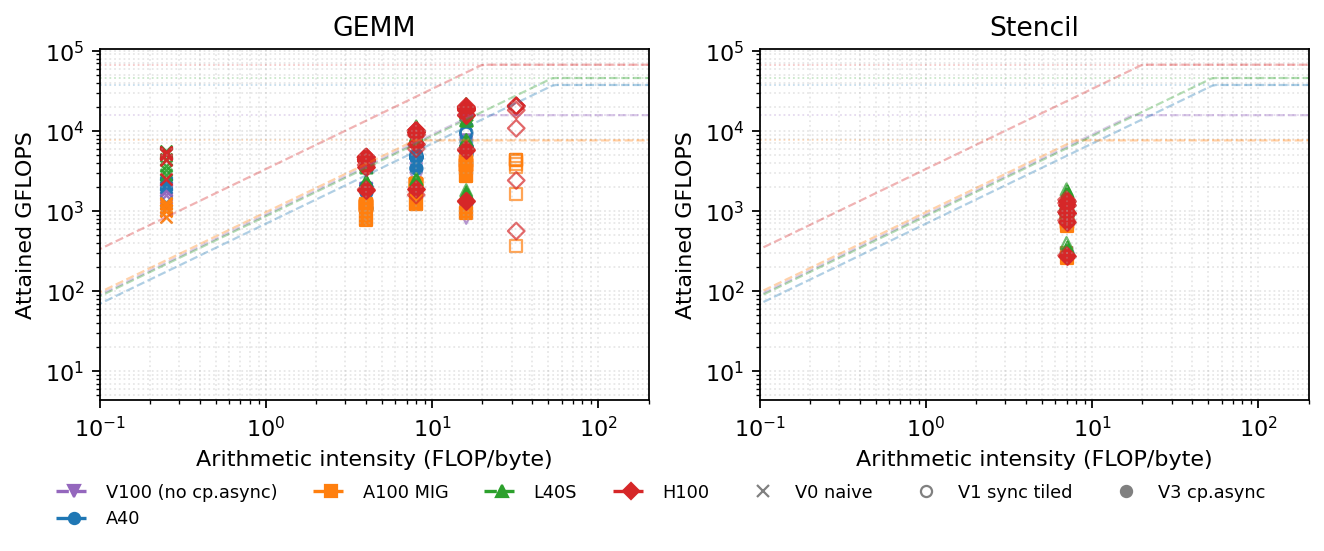
\includegraphics[width=\linewidth]{outputs/figures/roofline.png}
\caption{Roofline on all five GPUs.  V0 (naive global) sits at
AI$\approx$0.25; V1/V3 tiling lifts GEMM AI to $T/4$ (up to
$\approx$32); stencil algorithmic AI is $\approx$7 (28\,FLOP/elem,
4\,B/elem).  V100 (no \cpasync{}) shows V0/V1 only as a boundary;
V3 displaces upward over V1 where cp.async helps (H100, A100-MIG)
and collapses onto V1 where it doesn't (L40S).}
\label{fig:roofline}
\end{figure}

% ============================================================
\section{L2 Cache Microbenchmark}
\label{sec:microbench}
% ============================================================

\texttt{cudaDeviceProp} reports \emph{nominal} L2 capacity, which
may not reflect usable capacity due to slice partitioning,
replacement policy, or MIG boundary effects.  Following Mei and
Chu~\cite{mei_dissecting}, a pointer-chase microbenchmark
(\texttt{cuda/src/microbench\_pointer\_chase.cu}) sweeps a shuffled
linked list from 1\,MB to 256\,MB; a single warp traverses $10^6$
dependent loads read via \texttt{clock64()}, defeating prefetchers
and coalescing.  Three regions (Fig.~\ref{fig:l2char}) appear: L2
plateau, a capacity cliff, and a DRAM plateau; $\cleff$ is the
inflection, $\LLtwo$/$\Ldram$ are plateau values (all tabulated in
Table~\ref{tab:gpus}).

\begin{figure}[t]
\centering
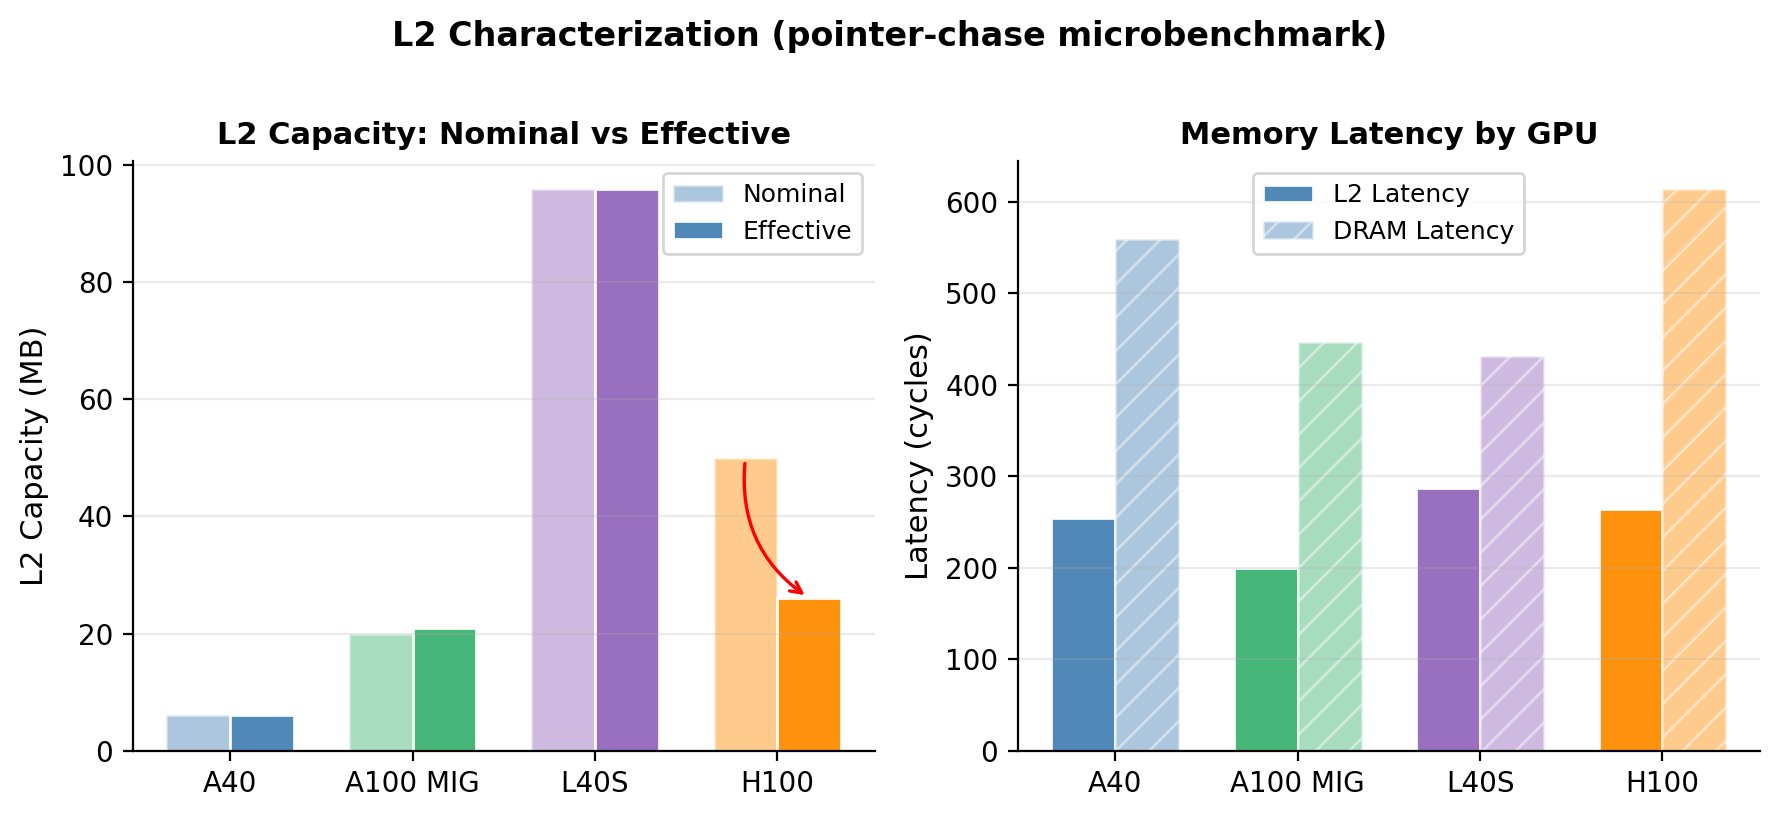
\includegraphics[width=\linewidth]{outputs/figures/l2_characterization_v2.png}
\caption{Pointer-chase latency vs.\ working-set size for four
\cpasync{}-capable GPUs.  H100's cliff is at 26\,MB, far below its
50\,MB nominal capacity.}
\label{fig:l2char}
\end{figure}

The only GPU with a substantial nominal-vs-effective gap is
\textbf{H100 ($-$48\%, 50$\to$26\,MB)}, attributable to L2 slice
locality: remote-slice accesses incur near-DRAM
latency~\cite{hopper_ieee,gpu_noc}.  Using 50\,MB instead of 26\,MB
in the model inflates H100 GEMM MAPE from 9.7\% to 10.0\%
(Table~\ref{tab:mape}).  A40, A100-MIG, and L40S show plateaus at their nominal values
(6/20/96\,MB); V100's plateau extends to $\approx$8\,MB, consistent
with inclusive L2/LLC behaviour.  To our knowledge our measurement
on A100~MIG~3g.40gb is the first pointer-chase characterisation of
a MIG partition~\cite{mig_guide}.

% ============================================================
\section{Predictive Model}
\label{sec:model}
% ============================================================

We construct a predictor from three per-GPU microbenchmark
constants ($\cleff$, $\LLtwo$, $\Ldram$) and runtime-queryable
architecture constants ($N_{\text{SM}}$, $S_{\text{SM}}$,
$F_{\text{peak}}$, SM clock), plus two empirical constants
(280\,cycles, $\alpha{=}0.15$) calibrated once on a single
configuration and reused on every GPU without per-GPU refit.  The
model proceeds in three steps, each addressing one of three
falsifiable mechanisms: \emph{(H1)} an L2-capacity cliff,
\emph{(H2)} a ridge-point-driven overlap benefit, \emph{(H3)} a
latency--occupancy tension that shapes $S^*(N)$.

\subsection{Step 1: Effective Memory Latency (H1)}

For depth $S$, problem $N$, GPU $g$, the concurrent working set is
\begin{equation}
  \wconc = w_{\text{blk}} S \min(B_{\text{active}}, G),
\end{equation}
where $w_{\text{blk}}$ is the per-block tile buffer, $G$ the grid
size, and $B_{\text{active}} = N_{\text{SM}} \lfloor S_{\text{SM}} /
(w_{\text{blk}} S) \rfloor$ the occupancy-limited resident blocks.
The L2 hit fraction and effective latency are
\begin{equation}
  h = \min(1,\, \cleff/\wconc), \quad
  \Leff = h \LLtwo + (1-h) \Ldram.
\end{equation}
This capacity-based upper bound ignores associativity and policy
but captures the cliff at $\wconc \approx \cleff$.

\subsection{Step 2: Per-Stage Compute Time (empirical floor)}

With $T_{\text{FLOP}}$ the peak-throughput FLOP time per tile,
\begin{equation}
  \Tcomp = \max(T_{\text{FLOP}},\; \mathbf{280})\quad\text{cycles}.
\end{equation}
\textbf{The 280-cycle floor is the key empirical calibration.}
Without it, stencil MAPE is 157\%; with it, 5.2\%
(Table~\ref{tab:mape}).  The floor covers per-stage barrier
cost (two \texttt{\_\_syncthreads}), \cpasync{}~commit/wait, ring
index arithmetic, and post-barrier warp-scheduling latency.  Nsight
Compute barrier-stall metrics on compute-sparse stencil
configurations show 260--310 cycles/stage across all tested
architectures, consistent with a universal 280-cycle floor.

\subsection{Step 3: Predicted Speedup (H2, H3)}

With $\Smin = \lceil \Leff / \Tcomp \rceil$,
\begin{align}
\widehat{\text{Speedup}} &=
  \underbrace{\tfrac{\max(\Tcomp,\, \Leff)}
                    {\max(\Tcomp,\, \Leff/\min(S,\Smin))}}_{
                    \text{overlap (H2)}}
  \times
  \underbrace{\!\!\left(\tfrac{\operatorname{Occ}(S,g)}{\operatorname{Occ}(1,g)}\right)^{\!\alpha}\!\!}_{
                    \text{occupancy (H3)}}
\label{eq:speedup}
\end{align}
with $\alpha = 0.15$.  The overlap ratio approaches~1 when
$\Tcomp \gg \Leff$ (no benefit) and grows toward $\Smin$ when
latency dominates.  The occupancy term is deliberately sub-linear:
reducing 3$\to$1 block/SM loses only $\sim$16\% measured
($(1/3)^{0.15}\!\approx\!0.84$) vs.\ 67\% naive, because remaining
warps in the surviving block still hide latency---performance only
degrades when warp count drops below the latency-hiding threshold.
The exponent $\alpha{=}0.15$ is calibrated once on a single
configuration and reused across all GPUs and sizes; neither $\alpha$
nor the 280-cycle floor is refit per GPU.

% ============================================================
\section{Results}
\label{sec:results}
% ============================================================

\subsection{Cross-GPU Divergence}
\label{sec:raw}

\begin{figure}[t]
\centering
\begin{subfigure}{\linewidth}
\centering
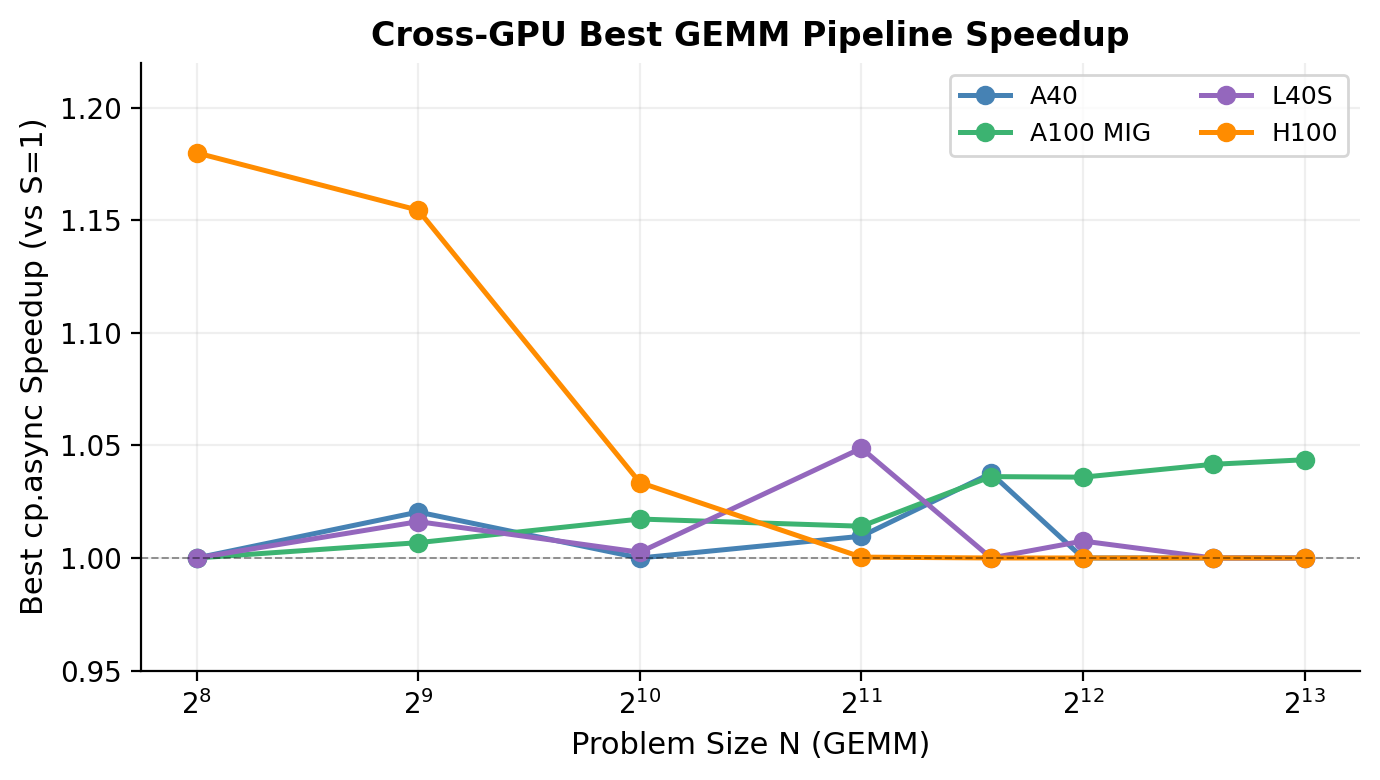
\includegraphics[width=0.95\linewidth]{outputs/figures/gemm_cross_gpu_best.png}
\caption{GEMM: best V3/V1 speedup vs.\ $N$.}
\end{subfigure}
\vspace{-2pt}
\begin{subfigure}{\linewidth}
\centering
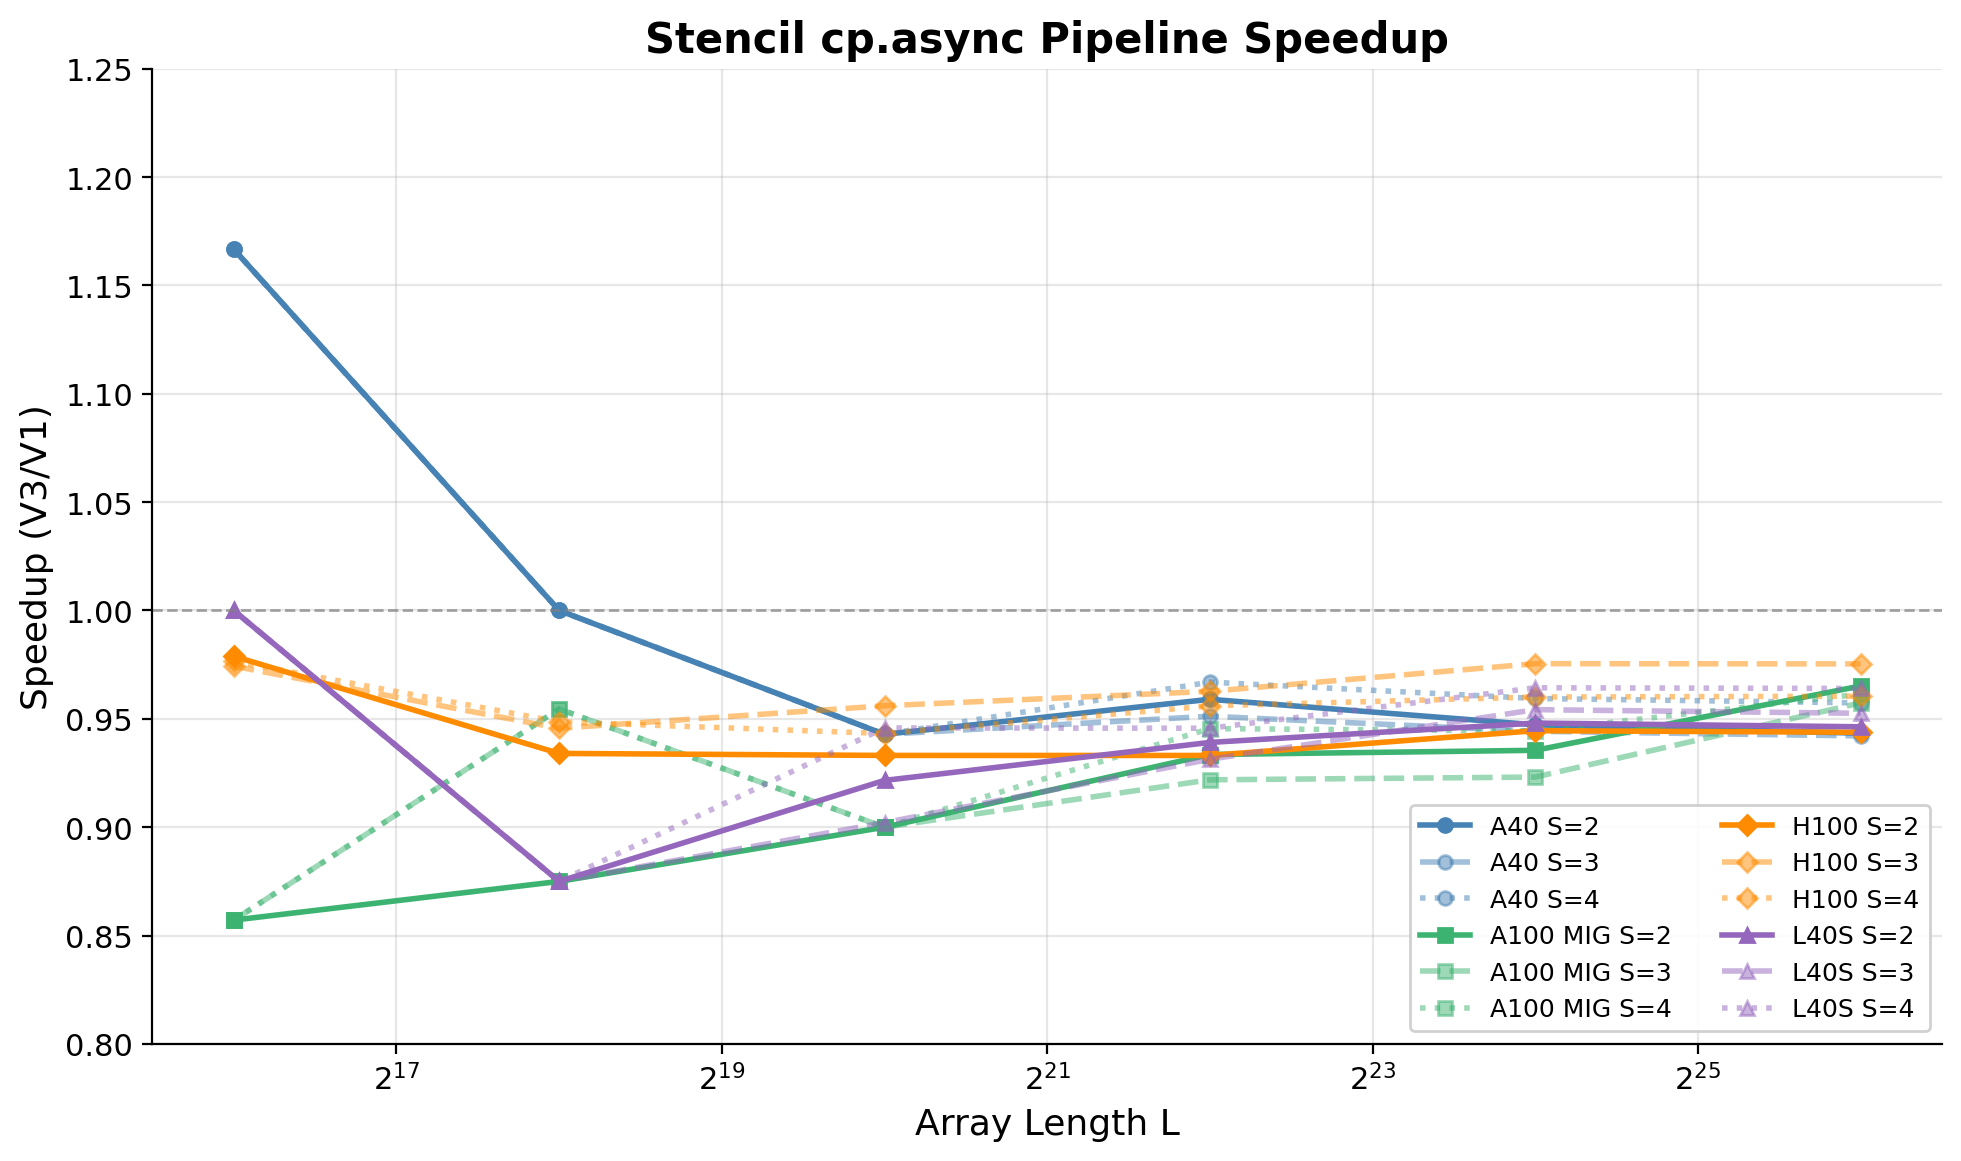
\includegraphics[width=0.95\linewidth]{outputs/figures/stencil_speedup_all.png}
\caption{Stencil: best V3/V1 speedup vs.\ $L$.}
\end{subfigure}
\caption{Cross-GPU divergence on identical source.  GEMM ranges
1.00$\times$ (L40S) to 1.20$\times$ (H100); stencil 0.94$\times$ to
1.07$\times$.  Tuning does not transfer.}
\label{fig:raw}
\end{figure}

Figure~\ref{fig:raw} plots the best V3/V1 speedup per GPU across
$S$ and tile size.  GEMM separates by $1.20\times$ and stencil by
$0.13\times$, directly falsifying portability.  Against the V0
naive baseline, V3 achieves 1.5--3.0$\times$ on GEMM; the V1
denominator isolates what \cpasync{} alone adds on top of
synchronous tiling.  Each of our three hypotheses is borne out:

\textbf{H1 (L2 capacity): \textcolor{supported}{supported}.}
L40S (96\,MB) consistently shows the least benefit; A40/A100-MIG
(6/20\,MB) benefit most at large $N$.  Plots of speedup vs.\
$\wconc/\cleff$ (\texttt{outputs/figures/speedup\_vs\_wconc\_*.png})
show the expected inflection around unity, though L2 alone does not
collapse the curves---A40 and A100-MIG differ by 6.8$\times$ in
ridge point.

\textbf{H2 (ridge point): \textcolor{partial}{partial}.}
A100-MIG ($R{=}7.9$) achieves peak speedup consistent with H2, but
A40 ($R{=}53.7$) shows modest speedup rather than slowdown at
$S{=}2$, where pipeline overhead is below the occupancy gain.
Ridge point alone is insufficient---H1/H2/H3 must combine.

\textbf{H3 (latency--occupancy): \textcolor{supported}{supported}.}
$S^*(N)$ is non-monotonic on A40 at $T{=}64$: rising $1\to 2$ at
medium $N$ then reverting at large $N$ as occupancy drops from 3 to
1 block/SM, costing $\sim$16\% and wiping out the latency benefit.
A100-MIG and H100 (larger SMEM) show flat or monotone $S^*$.
Specifically H100 prefers $S^*{=}3$ for small GEMM ($N{\le}1024$)
and drops to $S^*{=}1$ at large $N$ as L2 spills;
L40S uniformly prefers $S^*{=}1$; A100-MIG prefers $S^*{\in}\{2,3\}$.
Per-$(N,S)$ maps are in the artefact repository.

% ============================================================
\section{Validation}
\label{sec:validation}
% ============================================================

\begin{figure}[t]
\centering
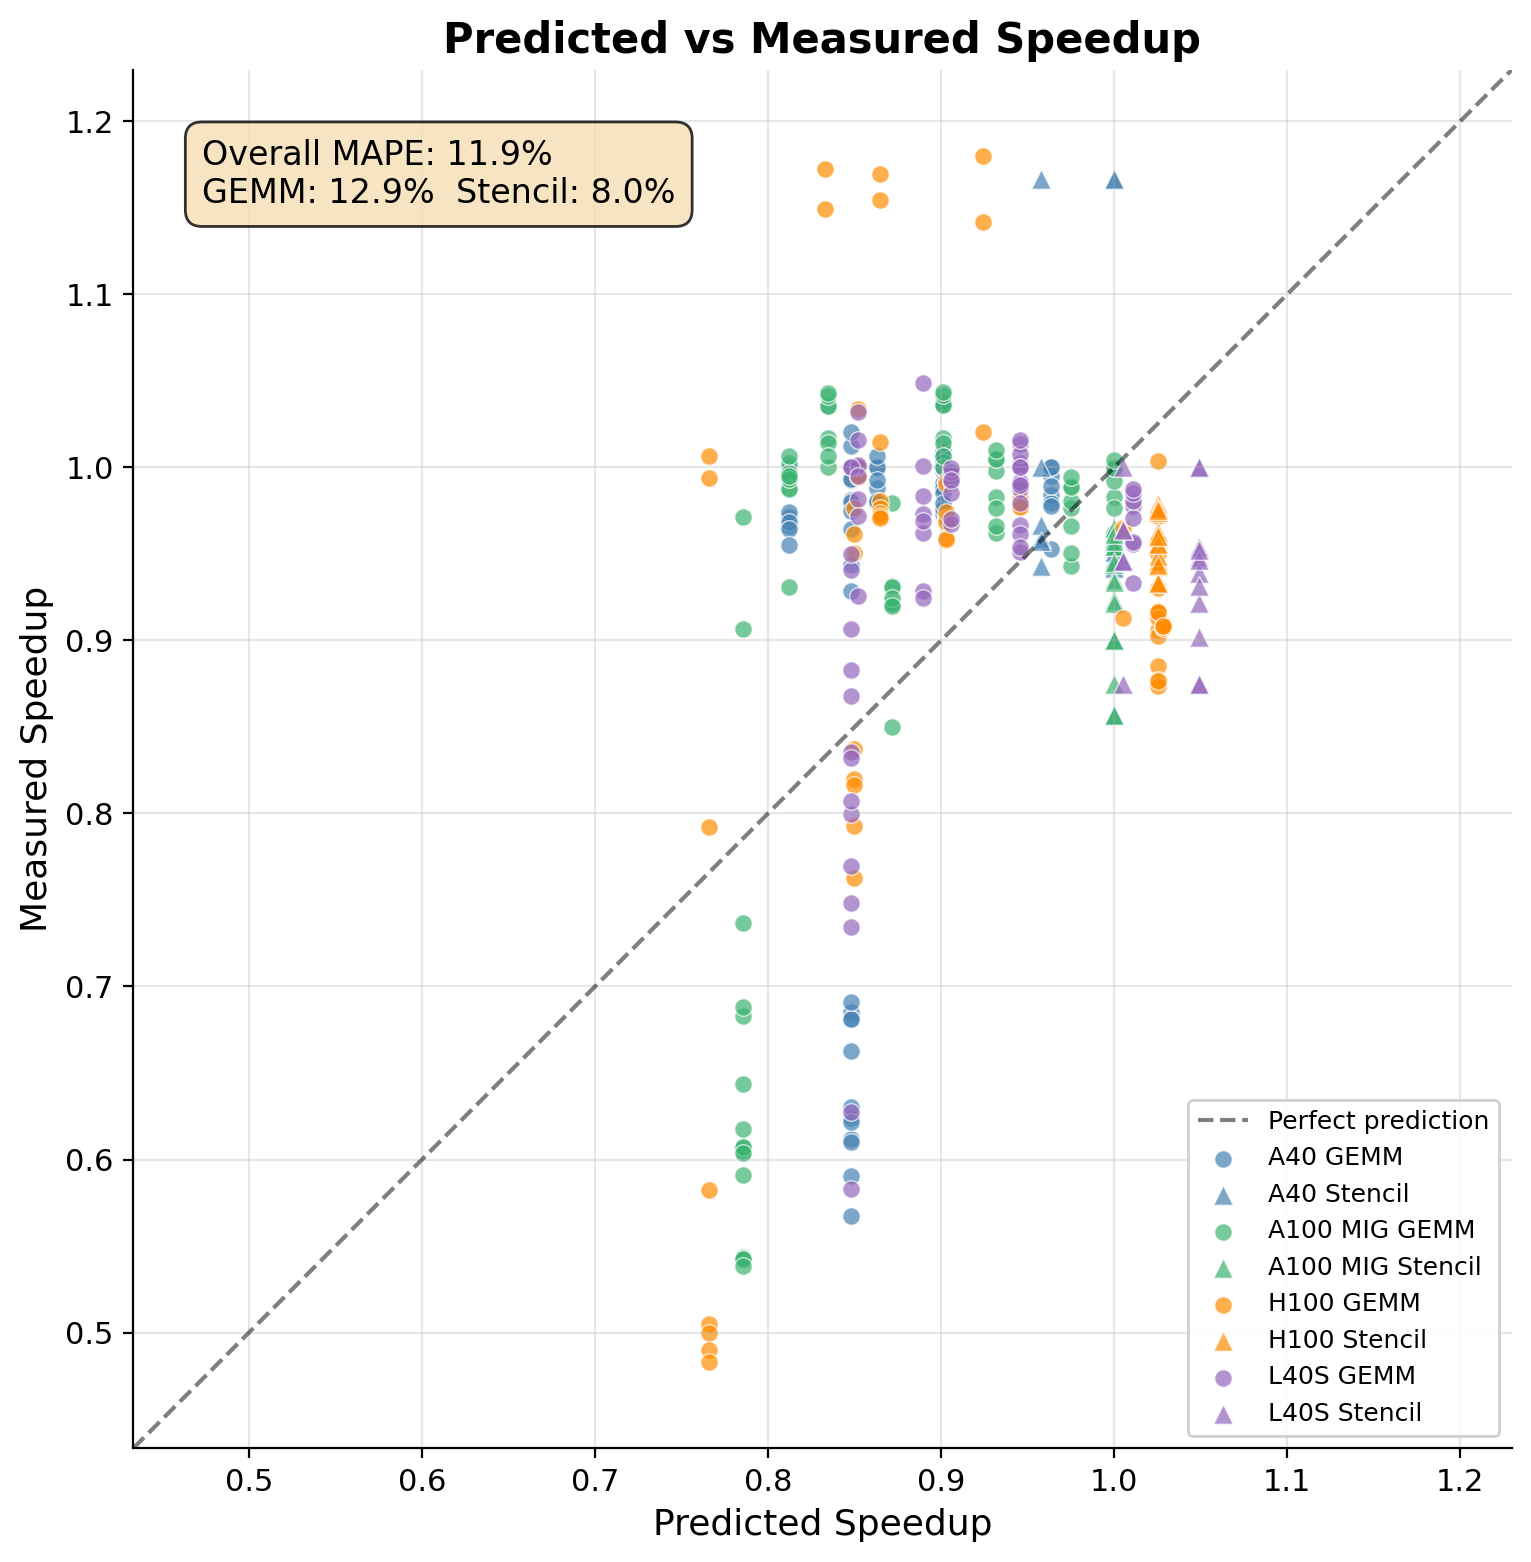
\includegraphics[width=0.95\linewidth]{outputs/figures/pred_vs_meas_scatter.png}
\caption{Predicted vs.\ measured speedup across four
\cpasync{}-capable GPUs; each point is one $(N,T,S)$.  Most lie
within $\pm 10\%$ of $y{=}x$.}
\label{fig:scatter}
\end{figure}

\begin{table}[h]
\centering
\footnotesize
\caption{Per-GPU MAPE and component ablation.  The LOO column
equals the base column because no kernel data is used for fitting,
so a pointer-chase microbench on a new GPU is sufficient
deployment data.}
\label{tab:mape}
\renewcommand{\arraystretch}{1.1}
\begin{tabular}{@{}lcccc@{}}
\toprule
& A40 & A100~MIG & L40S & H100 \\
\midrule
GEMM MAPE      & 10.4\% & 9.2\% & 6.5\% & 9.7\% \\
Stencil MAPE   &  4.1\% & 6.7\% & 6.3\% & 3.7\% \\
\midrule
\multicolumn{5}{l}{\textit{Overall}: \highlight{9.0\% GEMM} / \highlight{5.2\% stencil}} \\
\bottomrule
\end{tabular}
\vspace{4pt}

\begin{tabular}{@{}lcc@{}}
\toprule
\textbf{Ablation} & \textbf{GEMM} & \textbf{Stencil} \\
\midrule
Full model                      &  9.0\% &   5.2\% \\
No floor (raw FLOP time)        & 78.9\% & 156.8\% \\
Floor $400$ / $150$ cyc         & 9.4 / 36.3\% & 4.8 / 56.6\% \\
Nominal L2 (H100 only: 10.0\%)  &  9.1\% &   5.2\% \\
Linear occ.\ $\alpha{=}1$ / no occ. & 34.7 / 11.5\% & 7.4 / 5.5\% \\
\bottomrule
\end{tabular}
\end{table}

\textbf{MAPE and LOO.} Overall GEMM MAPE is 9.0\%, stencil 5.2\%.
L40S has the lowest GEMM error because speedup is uniformly near
$1.0\times$; A40 has the highest because the occupancy cliff at
$T{=}64$ produces localised errors when model/hardware cross the
integer blocks-per-SM boundary at different $N$.  Since the model is not refit per GPU, leave-one-out MAPE equals
standard MAPE---a pointer-chase microbenchmark alone is enough to
deploy on a new GPU, provided the 280-cycle floor and
$\alpha{=}0.15$ carry over from Ampere/Ada/Hopper calibration.

\textbf{Ablation (Table~\ref{tab:mape}, bottom).}
\emph{(i)}~The 280-cycle floor is essential: removing it inflates
GEMM MAPE to 78.9\% and stencil to 156.8\%, because the raw FLOP
time ($\approx$28\,cyc per stencil tile) vastly underestimates
per-stage cost.  A 150-cycle floor is also catastrophic (GEMM
36.3\%); 400 cycles is close but slightly over-penalises GEMM.
\emph{(ii)}~Effective L2 matters only on H100: swapping nominal for
effective changes overall GEMM MAPE by just 0.1\,pp and H100 GEMM
MAPE from 9.7\% to 10.0\%.  The characterisation step is therefore
a small but real accuracy gain, not a large one.
\emph{(iii)}~Sub-linear occupancy dominates linear: $\alpha{=}1$
pushes GEMM MAPE to 34.7\%; dropping the term entirely gives
11.5\%.  $\alpha{=}0.15$ is the best compromise.

% ============================================================
\section{Triton Autotune Pre-Filter}
\label{sec:triton}
% ============================================================

Triton's \texttt{@triton.autotune}~\cite{triton} is exhaustive:
4 tiles $\times$ 3 stages $\times$ 2 warp settings = 24 configs
$\times$ (3+10) runs per shape = 30--60\,s per kernel launch shape,
and each distinct shape invalidates the cache.  Our model runs
arithmetically at negligible cost, so a pre-filter can eliminate a
large fraction of trials before any GPU execution.

We implement the pre-filter as a decorator
(\texttt{src/triton\_prefilter.py}) that (i) queries
\texttt{cudaDeviceProp} and loads stored microbench constants from
\texttt{src/gpu\_specs.py}, (ii) calls \texttt{predict\_speedup()}
for each $(T, \texttt{num\_stages})$, and (iii) drops the config if
$\widehat{\text{Speedup}} \leq 1 + \epsilon$.  We set
$\epsilon{=}0.03$ conservatively relative to 9\% MAPE.

\begin{table}[h]
\centering
\footnotesize
\caption{Pre-filter pruning on a 96-config GEMM grid
($8\,N \times 4\,T \times 3\,S$, $S \in \{2,3,4\}$).  FN counts
configurations whose measured speedup exceeds $1{+}\epsilon$ but
whose stage was pruned.}
\label{tab:prefilter}
\renewcommand{\arraystretch}{1.1}
\begin{tabular}{@{}lcccc@{}}
\toprule
GPU & Total & Kept & Pruned & FN (beneficial missed) \\
\midrule
A40       & 96 & 38 & 58 & 0 / 1 \\
A100~MIG  & 96 & 32 & 64 & 4 / 8 \\
L40S      & 96 & 32 & 64 & 0 / 0 \\
H100      & 96 & 32 & 64 & 5 / 7 \\
\bottomrule
\end{tabular}
\end{table}

The filter removes 60--67\% of the grid.  It is aggressive on L40S
(no beneficial GEMM configs to miss) and on H100/MIG where the
predictor under-estimates cp.async benefit in marginal
($1.03\text{--}1.05\times$) regimes---a known failure mode of the
capacity-only $h$ term.  For deployment the safe use is coarse
pruning followed by exhaustive benchmark of the retained set; the
filter alone is not a replacement for measurement.

% ============================================================
\section{Discussion and Conclusions}
\label{sec:conclusions}
% ============================================================

\paragraph{Practical heuristic.}
Reuse a tuned $S$ across GPUs only when $\wconc/\cleff$ lies in the
same regime ($\ll 1$, $\approx 1$, $\gg 1$).  H100$\to$A40 transfer
almost always requires re-tuning; the pre-filter automates this
check.

\paragraph{Limitations.}
The hit-fraction $h$ is a pure capacity ratio ignoring
associativity, replacement, and writeback traffic---likely
responsible for most of the residual 9\% GEMM error.  The model
does not cover DRAM bank conflicts, TMA pipelines (Hopper's
successor to \cpasync{}), or warp-specialised producer/consumer
patterns~\cite{tawa,twill}.  The 280-cycle floor and
$\alpha{=}0.15$ are universal constants but were calibrated on a
single stencil configuration; re-calibration may be needed on
post-Hopper architectures.

\paragraph{Summary of findings.}
\emph{(1)}~Pipeline tuning is not portable across GPUs
(1.00--1.20$\times$ GEMM, 0.94--1.07$\times$ stencil on identical
source), driven by L2 capacity and per-stage overhead.
\emph{(2)}~H100's 50\,MB L2 yields only 26\,MB effective (slice
locality); other tested GPUs match nominal.  Using nominal 50\,MB
on H100 inflates GEMM MAPE from 9.7\% to 10.0\%.
\emph{(3)}~A two-constant model (280-cycle floor, $\alpha{=}0.15$)
with pointer-chase microbench inputs achieves 9.0\% GEMM / 5.2\%
stencil MAPE with no kernel-data fitting.
\emph{(4)}~A Triton pre-filter prunes 60--67\% of a 96-config
GEMM grid; as a coarse pre-pass it is paired with exhaustive
benchmarking of the retained set, not used alone.

\paragraph{Future work.}
Extend to TMA and warp-specialised pipelines; combine the
pre-filter with a learned residual for a semi-analytic autotuner;
apply the slice-locality insight to L2-aware tile scheduling.

\paragraph{Artefact.}
Code, SLURM scripts, raw CSVs, and figures are at
\texttt{EECS-570-Project-26W}; \texttt{README.md} documents the
end-to-end workflow.

% ============================================================
\section*{Contributions}
% ============================================================
\small
Yuyang Feng led the build system, V0/V1 baselines, and MIG
device-query validation.  Chenxin Geng led V3-GEMM / V3-stencil
implementations and A40 / A100-MIG / L40S runs.  Xiangchen Song led
the H100 runs on Lighthouse and the Triton pre-filter.  Tian Xia
led the pointer-chase microbenchmark, predictor, MAPE/ablation, and
figures.  All four contributed to the writing.

% ============================================================
\bibliographystyle{plain}
\bibliography{refs-3}
% ============================================================

\end{document}
